\documentclass{article} %We will probably want to change this document class
\usepackage{amsmath}
\usepackage{amsfonts}
\usepackage{amsthm}
\usepackage{amssymb}
\usepackage{attachfile} %Lets me embed whatever I want
\usepackage{graphicx} %Allows us to print pictures
\usepackage[a4paper]{geometry} %Adjusts margins
%Note:Those who want to read on tablets or other handheld digital devices need to create documents without the extra whitespace. In order to create PDF documents with optimal handheld viewing, not only must the text field and margins be adjusted, so must the page size. If you are looking for a sensible dimension, consider following the paper size used by the Supreme Court of the United States, 441pt by 666pt (or 6.125 inches by 9.25 inches), which looks great on tablets. You could also use the Supreme Court's text field size of 297 pt by 513 pt, but this is too wide for fonts other than Century Schoolbook, the font required by the Supreme Court.
\usepackage{enumerate} %numbered lists
\usepackage{multirow}
\usepackage{media9} %Allows embedding of media files
\usepackage{float} %Allows control over position of floating elements
\usepackage{units}
\usepackage[in]{fullpage}
\usepackage[small]{caption} %allows you to caption pictures
\numberwithin{equation}{section} %Numbers within equations within sections
\linespread{1.0} %Single Spaced
\graphicspath{ {./Examples/} }
\addmediapath{./Examples/}

\begin{document}

	\begin{center}
		\textbf{Harmonic Rhythm}\\
	\end{center}


		\textit{Harmonic rhythm} is a term used to describe the frequency of harmonic changes in music. It is the rate of chord change in relation to time. A song that calls for relatively few harmonic changes has a slow harmonic rhythm, while another song which calls for a lot of harmonic changes has a faster harmonic rhythm. \\

		The term \textit{harmonic rhythm} may be misleading because \textit{rhythm} is expressed by using notes of various durational values (half, quarter, and eighth notes) and has nothing to do with \textit{harmonic} rhythm. \\

		An understanding of harmonic rhythm is a necessity in successful barbershop arranging. But even more important is the \textit{perception} of the primary harmonic rhythm. \\

		The piano man who plays by ear-and who plays the right chords at the right time-has this perception of primary harmony. He may embellish .the basic harmony called for by the melody, but he never fails to make the essential chord changes at the right places. \\

		The barbershop ear singer who seems to feel what's coming next has this perception of the correct harmonic rhythm. He too may add other chords to the basic chord changes called for by the melody, but he always makes the right move at the right time. \\

		So in understanding harmonic rhythm-how often chord changes occur-we must at the same time be aware that. some harmonic changes are \textit{required} while some are added to increase interest or excitement. \\

		Since required harmonic changes are chord \textit{root} changes, perception of these primary `pillars'' or harmonic signposts is essential to the arranger. In the following example, observe the primary root (chord) changes: \\

		%Example 1
		\begin{figure}[H]
		\textbf{Example 1}
		
		\includemedia[
			addresource=Example1.mp3, %Name of the sound file I'm adding
			activate=onclick,
			flashvars={
				source=Example1.mp3
				&autoPlay=true
			},
			transparent
			]{\color{blue}\framebox[0.4\linewidth][c]{Listen}}{APlayer.swf}\\

		\textattachfile[print=false]{./Examples/Example1.mus}{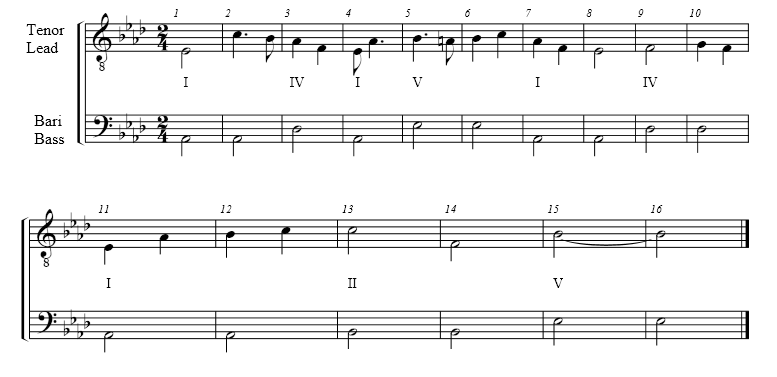
\includegraphics[width=\linewidth, keepaspectratio=true]{Example1.png}}\\
		\end{figure}

		The harmonic roots (bass notes) in Example 1 represent the primary chords which underlie the melody of this song. They are the minimum requirements necessary to provide adequate harmonic `accompaniment.'' But they are required! In an attempt to describe what has taken place, we say `the harmonic rhythm of the melody requires these root changes at these particular spots.'' \\

		Anyone who has sung this song in an unaccompanied barbershop quartet is immediately aware that the bass singer does considerably more than shown in Example 1, and that substitute chords are used to harmonize melody notes that are `out of the primary chords.'' But the important thing is that the downbeats of measures 1, 3,4, 5, 7, 9, 11, 13 and 15, are the points of primary harmonic change. Any arrangement of this song has to observe those changes at those points or it won't sound like `Wait Till The Sun Shines, Nellie.'' \\

		In the arrangement published by the Society, observe that while there is \textit{more} harmonic activity than the minimum required by the harmonic rhythm of the song, all the primary changes have occurred at the points where the harmonic rhythm requires that they do:\\

		%Example 2
		\begin{figure}[H]
		\textbf{Example 2}
		
		\includemedia[
			addresource=Example2.mp3, %Name of the sound file I'm adding
			activate=onclick,
			flashvars={
				source=Example2.mp3
				&autoPlay=true
			},
			transparent
			]{\color{blue}\framebox[0.4\linewidth][c]{Listen}}{APlayer.swf}\\

		\textattachfile[print=false]{./Examples/Example2.mus}{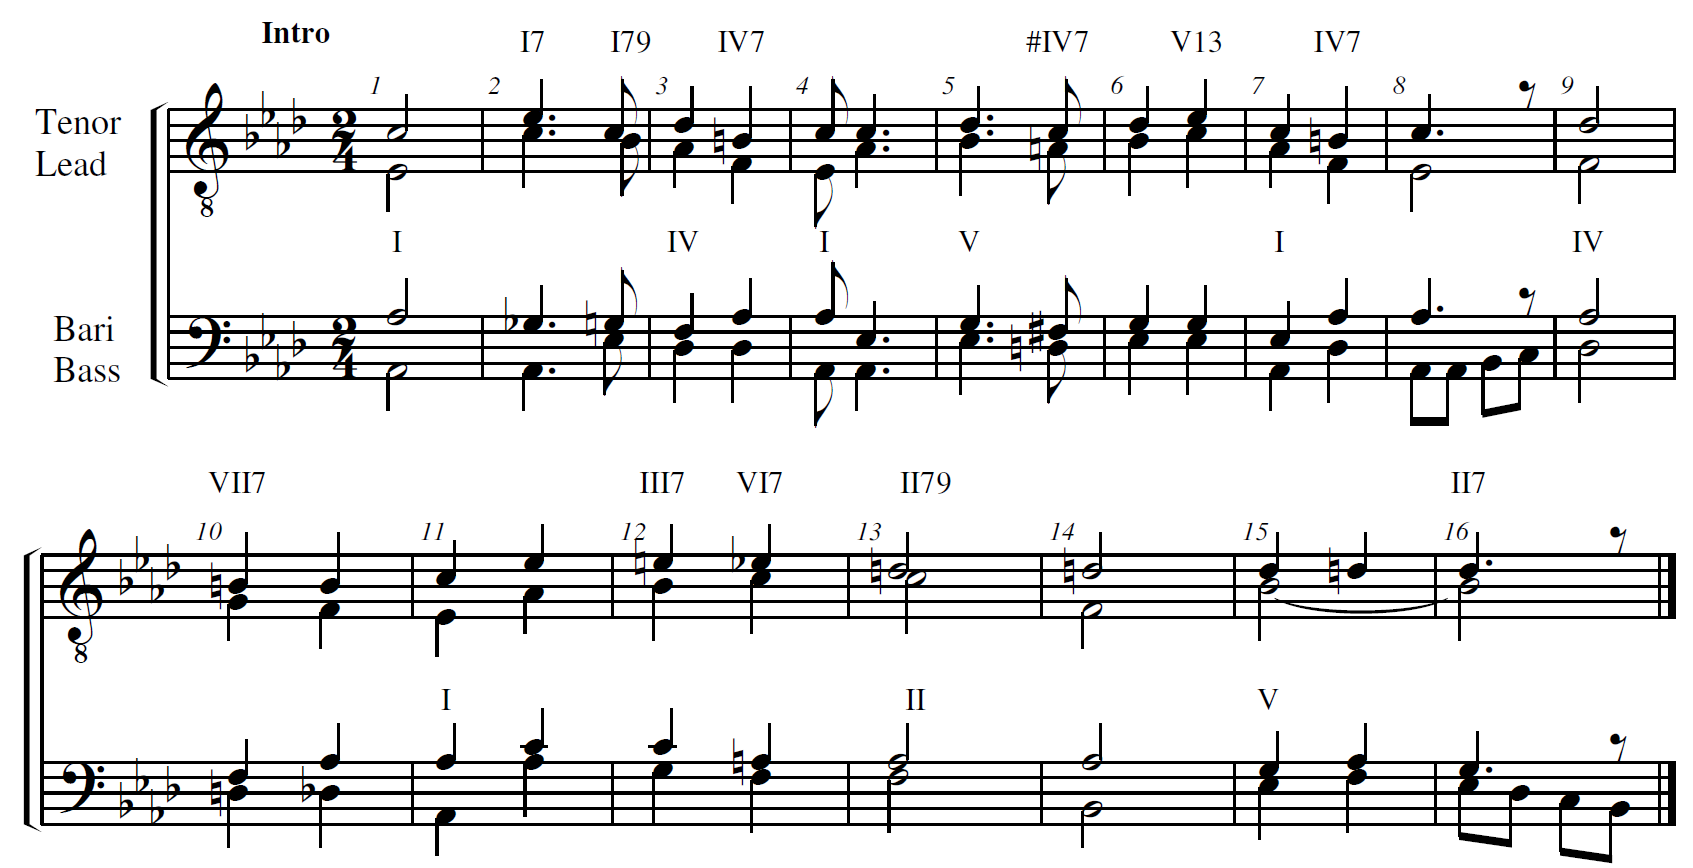
\includegraphics[width=\linewidth, keepaspectratio=true]{Example2.png}}\\
		\end{figure}

		The determination of primary harmony (roots) is the result of correct analysis of harmonic rhythm and, as pointed out in the chapter on `Barbershop Harmonization,'' becomes the basic harmonic foundation on which we build a barbershop arrangement. \\

		As stated earlier, harmonic rhythm is how often harmonic changes occur. In fast or up-tempo songs, there tend to be fewer harmonic changes, so we could say that generally, `\textit{fast} songs have \textit{slower} harmonic rhythm.'' In the next example, one chord root is sufficient to harmonize several measures: \\

		%Example 3
		\begin{figure}[H]
		\textbf{Example 3}
		
		\includemedia[
			addresource=Example3.mp3, %Name of the sound file I'm adding
			activate=onclick,
			flashvars={
				source=Example3.mp3
				&autoPlay=true
			},
			transparent
			]{\color{blue}\framebox[0.4\linewidth][c]{Listen}}{APlayer.swf}\\

		\textattachfile[print=false]{./Examples/Example3.mus}{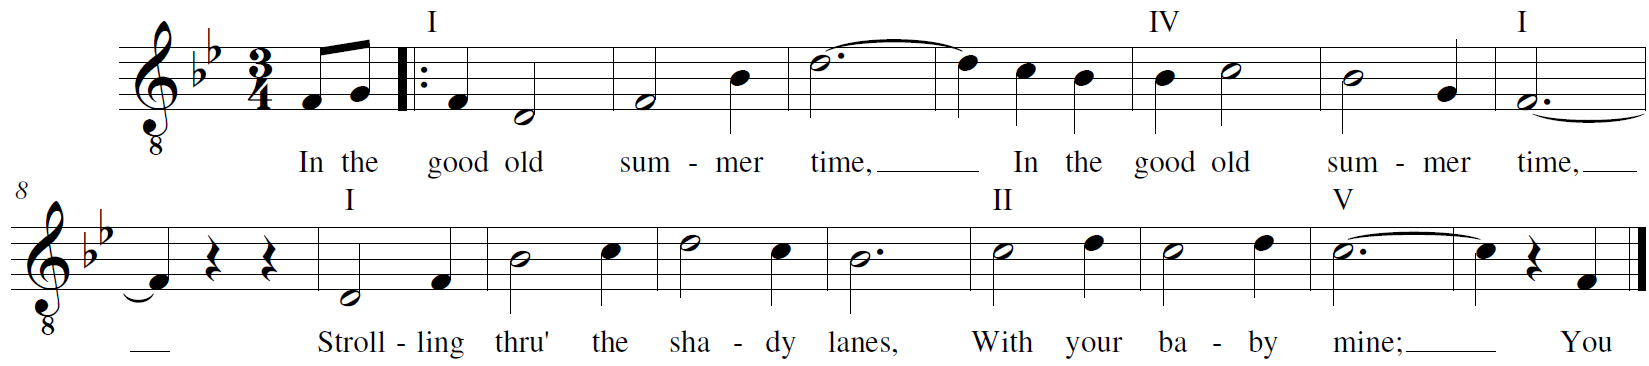
\includegraphics[width=\linewidth, keepaspectratio=true]{Example3.png}}\\
		\end{figure}

		\textit{It might be appropriate to point out that songs with extremely slow harmonic rhythm are often not well suited to barbershop. One chord root under a long phrase restricts the arranger and we perceive a lack of `harmonic variety.''} \\

		The more chord changes required by the melody or imposed by the arranger, the more difficult an arrangement becomes to perform at a fast tempo. Many ballads tend to have more cbord changes, so we could say that generally, `\textit{slow} songs have \textit{faster} harmonic rhythm.'' In the song `Sweet Adeline,'' chord changes occur on some consecutive melody notes within a single measure: \\

		%Example 4
		\begin{figure}[H]
		\textbf{Example 4}
		
		\includemedia[
			addresource=Example4.mp3, %Name of the sound file I'm adding
			activate=onclick,
			flashvars={
				source=Example4.mp3
				&autoPlay=true
			},
			transparent
			]{\color{blue}\framebox[0.4\linewidth][c]{Listen}}{APlayer.swf}\\

		\textattachfile[print=false]{./Examples/Example4.mus}{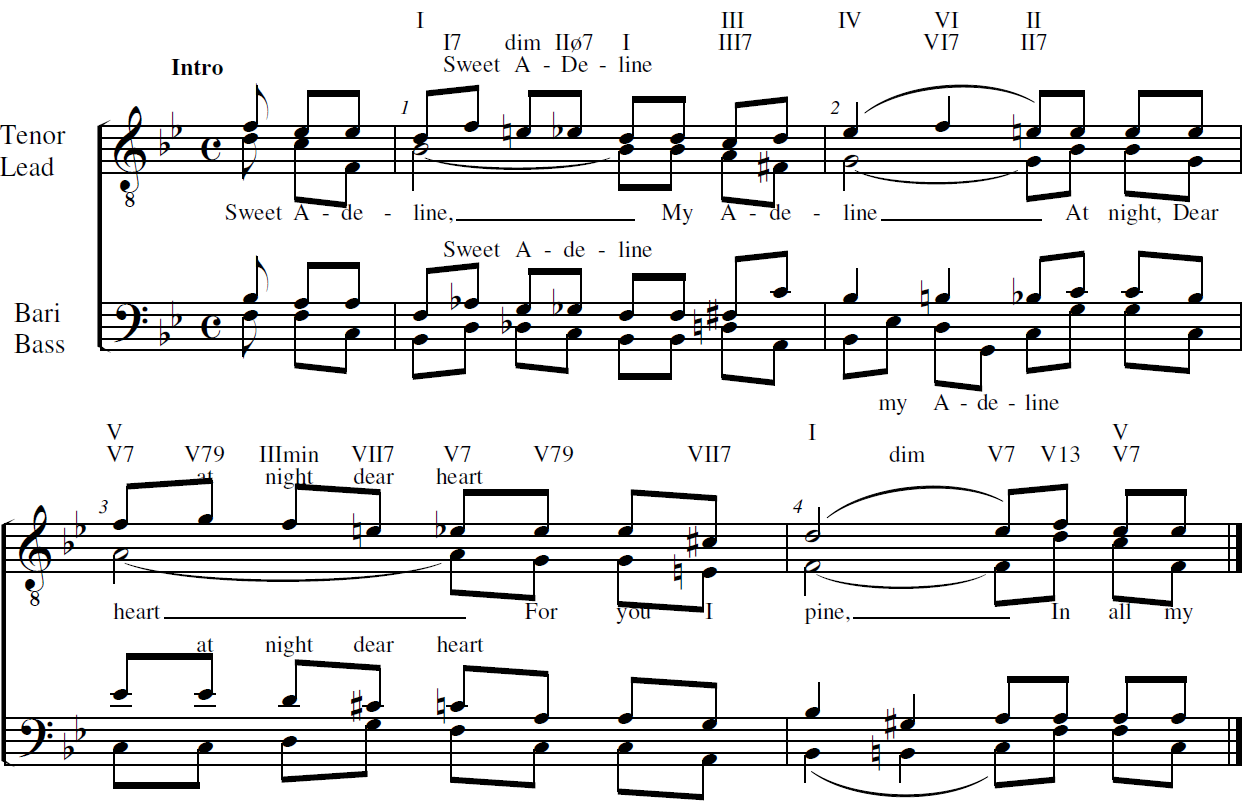
\includegraphics[width=\linewidth, keepaspectratio=true]{Example4.png}}\\
		\end{figure}

		The frequency of primary root changes is not necessarily consistent. In many songs, the rate of chord change accelerates toward the end of some phrases, thus generating a subtle increase in interest, emotional intensity, or excitement The next example shows a fairly slow harmonic rhythm to start with, becoming faster toward the end to give a more climactic feeling: \\

		%Example 5
		\begin{figure}[H]
		\textbf{Example 5}
		
		\includemedia[
			addresource=Example5.mp3, %Name of the sound file I'm adding
			activate=onclick,
			flashvars={
				source=Example5.mp3
				&autoPlay=true
			},
			transparent
			]{\color{blue}\framebox[0.4\linewidth][c]{Listen}}{APlayer.swf}\\

		\textattachfile[print=false]{./Examples/Example5.mus}{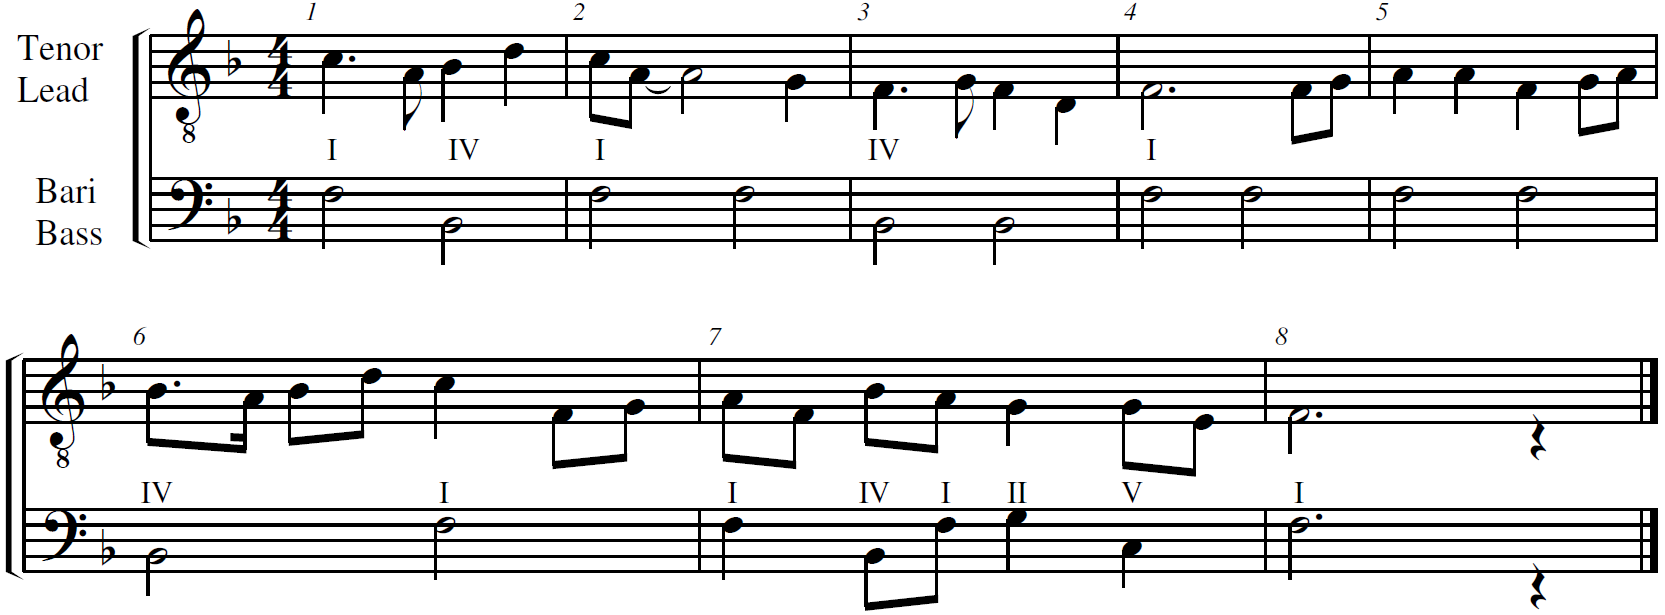
\includegraphics[width=\linewidth, keepaspectratio=true]{Example5.png}}\\
		\end{figure}

		Sometimes the frequency of chord change produce discernible patterns, though rarely as obviously as in this next example. Here, the harmonic rhythm of the melody seems to imply a root (chord) change every second measure: \\

		%Example 6
		\begin{figure}[H]
		\textbf{Example 6}
		
		\includemedia[
			addresource=Example6.mp3, %Name of the sound file I'm adding
			activate=onclick,
			flashvars={
				source=Example6.mp3
				&autoPlay=true
			},
			transparent
			]{\color{blue}\framebox[0.4\linewidth][c]{Listen}}{APlayer.swf}\\

		\textattachfile[print=false]{./Examples/Example6.mus}{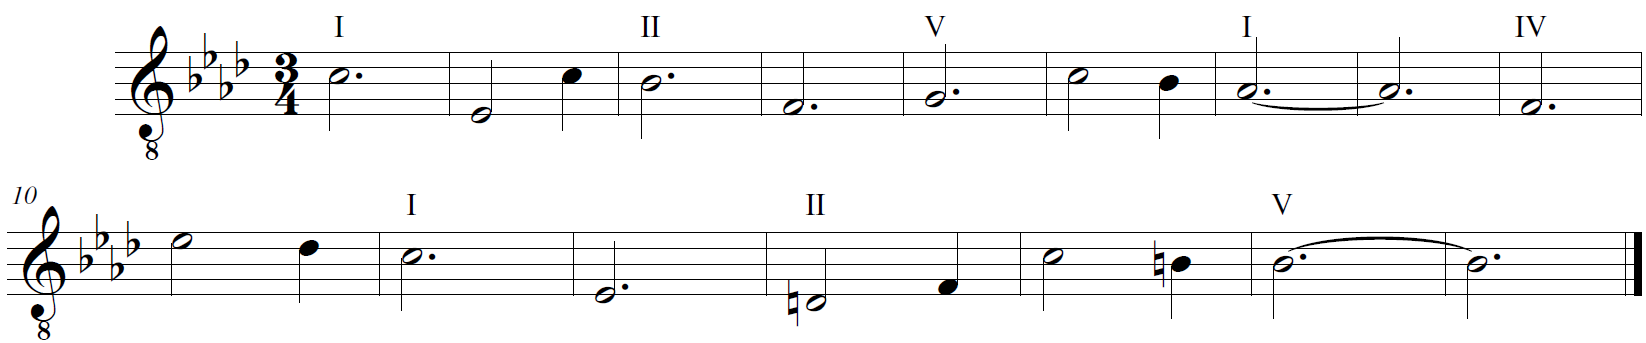
\includegraphics[width=\linewidth, keepaspectratio=true]{Example6.png}}\\
		\end{figure}

		Primary harmonic changes usually occur on strong beats of measures. In 2/4 and 3/4, important chord changes generally take place on the downbeat, while in 4/4 time, changes usually occur on the fIrst and third beats. While we see this important principle in ballads, it is specially true in faster songs, where the melodic structure almost always calls for harmonic changes on strong beats. \\

		In the next example, the `proper'' change of harmony occurs on strong beats. Compare with chord change that is `too late'' or `too soon.'' \\

		%Example 7
		\begin{figure}[H]
		\textbf{Example 7}
		
		\includemedia[
			addresource=Example7.mp3, %Name of the sound file I'm adding
			activate=onclick,
			flashvars={
				source=Example7.mp3
				&autoPlay=true
			},
			transparent
			]{\color{blue}\framebox[0.4\linewidth][c]{Listen}}{APlayer.swf}\\

		\textattachfile[print=false]{./Examples/Example7.mus}{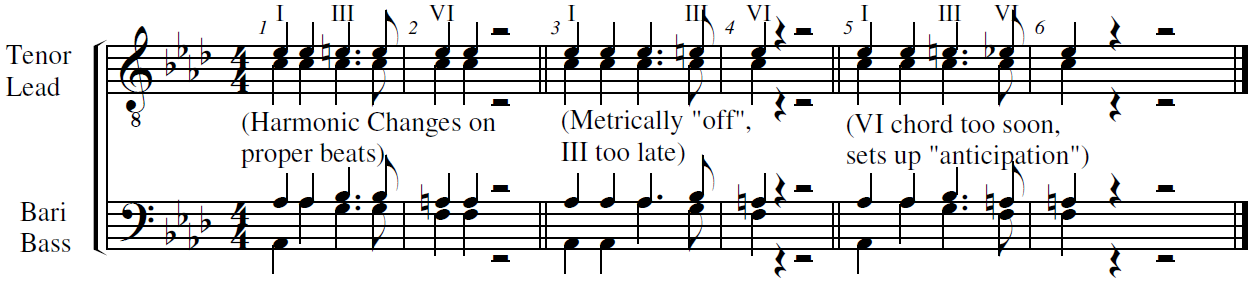
\includegraphics[width=\linewidth, keepaspectratio=true]{Example7.png}}\\
		\end{figure}

		So whenever the arranger has a choice, he should make chord changes on accented beats: \\

		%Example 8
		\begin{figure}[H]
		\textbf{Example 8}
		
		\includemedia[
			addresource=Example8.mp3, %Name of the sound file I'm adding
			activate=onclick,
			flashvars={
				source=Example8.mp3
				&autoPlay=true
			},
			transparent
			]{\color{blue}\framebox[0.4\linewidth][c]{Listen}}{APlayer.swf}\\

		\textattachfile[print=false]{./Examples/Example8.mus}{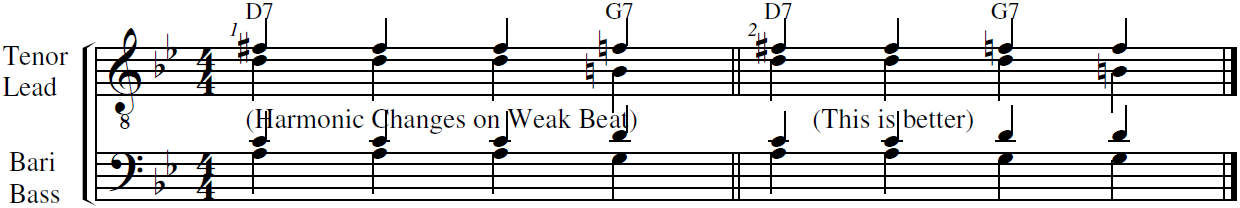
\includegraphics[width=\linewidth, keepaspectratio=true]{Example8.png}}\\
		\end{figure}

		If it is necessary to change harmony on a weak beat, change the harmony on the next strong beat if possible:\\

		%Example 9
		\begin{figure}[H]
		\textbf{Example 9}
		
		\includemedia[
			addresource=Example9.mp3, %Name of the sound file I'm adding
			activate=onclick,
			flashvars={
				source=Example9.mp3
				&autoPlay=true
			},
			transparent
			]{\color{blue}\framebox[0.4\linewidth][c]{Listen}}{APlayer.swf}\\

		\textattachfile[print=false]{./Examples/Example9.mus}{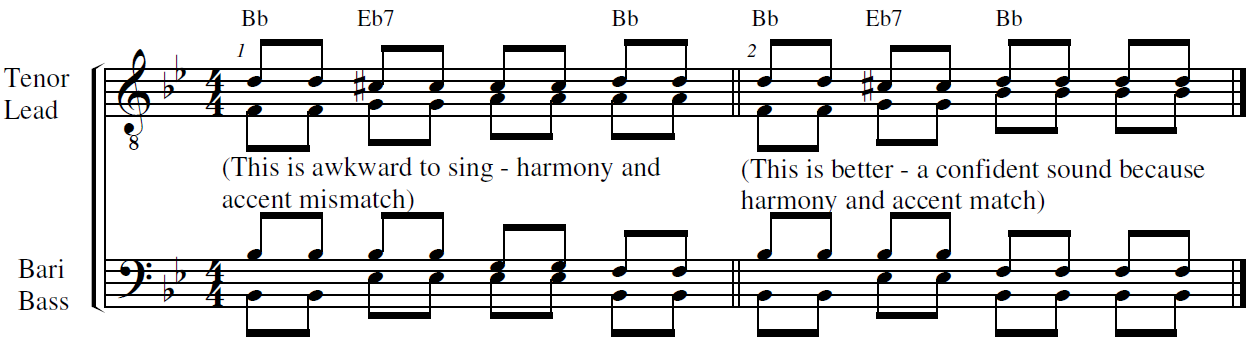
\includegraphics[width=\linewidth, keepaspectratio=true]{Example9.png}}\\
		\end{figure}

		If it becomes necessary to change harmony on the second half of a beat, change on the start of the next beat: \\

		%Example 10
		\begin{figure}[H]
		\textbf{Example 10}
		
		\includemedia[
			addresource=Example10.mp3, %Name of the sound file I'm adding
			activate=onclick,
			flashvars={
				source=Example10.mp3
				&autoPlay=true
			},
			transparent
			]{\color{blue}\framebox[0.4\linewidth][c]{Listen}}{APlayer.swf}\\

		\textattachfile[print=false]{./Examples/Example10.mus}{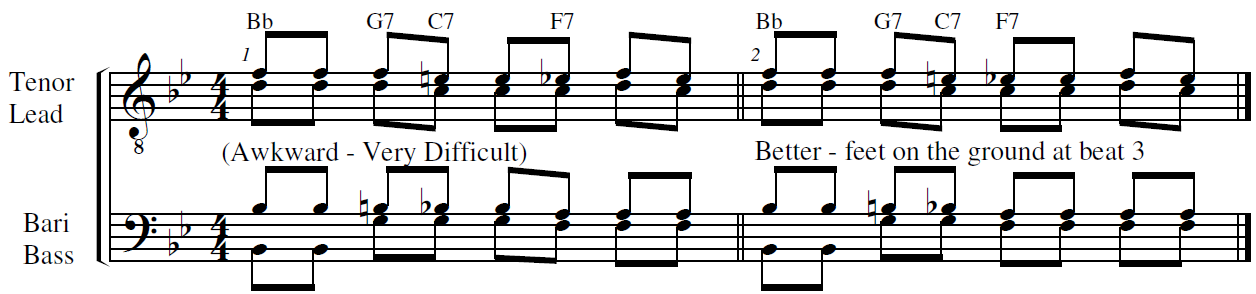
\includegraphics[width=\linewidth, keepaspectratio=true]{Example10.png}}\\
		\end{figure}

		\textit{Syncopation} is defined as `displacement or shifting of accents.'' The harmonic rhythm of a melody normally calls for harmonic change on strong beats, so when we encounter syncopated rhythm, we see the accent displaced: \\

		%Example 11
		\begin{figure}[H]
		\textbf{Example 11}
		
		\includemedia[
			addresource=Example11.mp3, %Name of the sound file I'm adding
			activate=onclick,
			flashvars={
				source=Example11.mp3
				&autoPlay=true
			},
			transparent
			]{\color{blue}\framebox[0.4\linewidth][c]{Listen}}{APlayer.swf}\\

		\textattachfile[print=false]{./Examples/Example11.mus}{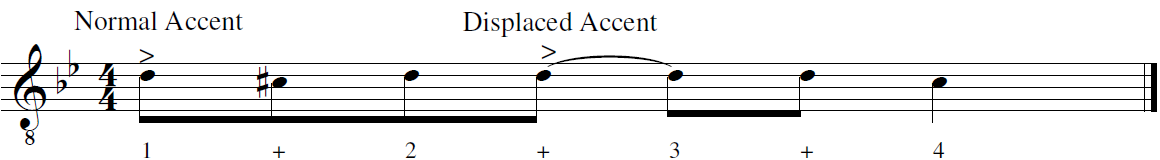
\includegraphics[width=\linewidth, keepaspectratio=true]{Example11.png}}\\
		\end{figure}

		Observe that in syncopation, the strong accents shift to an earlier beat or portion thereOf. The harmony must shift too, as in the next example: \\

		%Example 12
		\begin{figure}[H]
		\textbf{Example 12}
		
		\includemedia[
			addresource=Example12.mp3, %Name of the sound file I'm adding
			activate=onclick,
			flashvars={
				source=Example12.mp3
				&autoPlay=true
			},
			transparent
			]{\color{blue}\framebox[0.4\linewidth][c]{Listen}}{APlayer.swf}\\

		\textattachfile[print=false]{./Examples/Example12.mus}{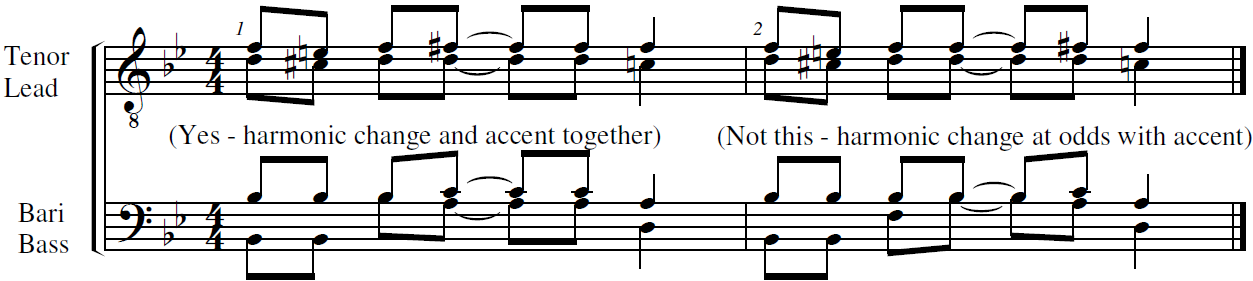
\includegraphics[width=\linewidth, keepaspectratio=true]{Example12.png}}\\
		\end{figure}

		We have seen. that \textit{frequency} of chord (root) change is called harmonic rhythm. We have also seen that the harmonic rhythm can be increased by appropriate use of additional chord changes' over the minimum required by the \textit{primary} harmonic rhythm. One other factor is important to the barbershop arranger: the kind of chord \textit{progression} generated by the harmonic rhythm of a melody. \\

		The best barbershop songs are those in which the harmonic rhythm suggests root movement on the Circle of Fifths. It is this kind of harmonic progression that we look for as arrangers of barbershop music. \\

		To sum up, the arranger must be aware of the primary harmonic pillars required by the harmonic rhythm-those chords that the melody implies \textit{must} be there---and they will ordinarily be on strong or accented beats. Additional harmonies may be employed to increase the harmonic rhythm, thus adding to the interest and excitement of the song, providing such additional chords still allow performance at proper tempo.\\


\end{document}